\documentclass[11pt]{article}
\usepackage[margin=1in]{geometry}
\usepackage{graphicx}
\usepackage{booktabs}
\usepackage{amsmath,amssymb}
\usepackage{array}
\usepackage{tabularx}
\usepackage[authoryear,round]{natbib}
\bibpunct{(}{)}{;}{a}{,}{,}
\setlength{\bibhang}{0.5in}
\setlength{\bibsep}{0pt}
\usepackage{xcolor}
\usepackage{caption}
\usepackage{tikz}
\usetikzlibrary{positioning,arrows.meta,shapes.geometric}
\usepackage[colorlinks=true,linkcolor=blue!50!black,citecolor=blue!50!black,urlcolor=blue!50!black]{hyperref}
\usepackage{setspace}
\onehalfspacing
\setlength{\parskip}{2pt}

% Every number in the text is generated by scripts/04 and 05 (generated/macros_leakage.tex); nothing is typed by hand.
\newcommand{\SubOnly}{0.580}
\newcommand{\SubOnlyLo}{0.565}
\newcommand{\SubOnlyHi}{0.594}
\newcommand{\TabNPath}{22,254}
\newcommand{\TabNCommon}{17,396}
\newcommand{\PureNPath}{16,903}
\newcommand{\PureNCommon}{1,479}
\newcommand{\PurePctPath}{76.0}
\newcommand{\PurePctCommon}{8.5}
\newcommand{\SampPurePctPath}{74.9}
\newcommand{\SampPurePctCommon}{7.9}
\newcommand{\NSample}{6,000}
\newcommand{\NPerClass}{3,000}
\newcommand{\MetaAll}{0.968}
\newcommand{\MetaAllLo}{0.963}
\newcommand{\MetaAllHi}{0.972}
\newcommand{\MetaHarm}{0.835}
\newcommand{\MetaHarmLo}{0.824}
\newcommand{\MetaHarmHi}{0.845}
\newcommand{\MetaFlag}{0.812}
\newcommand{\MetaFlagLo}{0.801}
\newcommand{\MetaFlagHi}{0.823}
\newcommand{\MetaTerms}{0.958}
\newcommand{\MetaTermsLo}{0.953}
\newcommand{\MetaTermsHi}{0.964}
\newcommand{\MetaShared}{0.624}
\newcommand{\MetaSharedLo}{0.609}
\newcommand{\MetaSharedHi}{0.637}
\newcommand{\DnbRef}{0.681}
\newcommand{\DnbRefLo}{0.668}
\newcommand{\DnbRefHi}{0.694}
\newcommand{\DnbDelta}{0.507}
\newcommand{\DnbDeltaLo}{0.492}
\newcommand{\DnbDeltaHi}{0.522}
\newcommand{\HynRef}{0.617}
\newcommand{\HynRefLo}{0.604}
\newcommand{\HynRefHi}{0.632}
\newcommand{\HynDelta}{0.524}
\newcommand{\HynDeltaLo}{0.508}
\newcommand{\HynDeltaHi}{0.537}
\newcommand{\KmRef}{0.568}
\newcommand{\KmRefLo}{0.554}
\newcommand{\KmRefHi}{0.583}
\newcommand{\KmDelta}{0.504}
\newcommand{\KmDeltaLo}{0.490}
\newcommand{\KmDeltaHi}{0.519}
\newcommand{\PureStratP}{2,247}
\newcommand{\PureStratC}{236}
\newcommand{\DnbRefPure}{0.749}
\newcommand{\DnbRefPureLo}{0.711}
\newcommand{\DnbRefPureHi}{0.782}
\newcommand{\DnbDeltaPure}{0.493}
\newcommand{\DnbDeltaPureLo}{0.455}
\newcommand{\DnbDeltaPureHi}{0.532}
\newcommand{\HynRefPure}{0.635}
\newcommand{\HynRefPureLo}{0.596}
\newcommand{\HynRefPureHi}{0.674}
\newcommand{\HynDeltaPure}{0.527}
\newcommand{\HynDeltaPureLo}{0.487}
\newcommand{\HynDeltaPureHi}{0.563}
\newcommand{\KmRefPure}{0.552}
\newcommand{\KmRefPureLo}{0.512}
\newcommand{\KmRefPureHi}{0.591}
\newcommand{\KmDeltaPure}{0.460}
\newcommand{\KmDeltaPureLo}{0.422}
\newcommand{\KmDeltaPureHi}{0.501}
\newcommand{\MetaPure}{0.582}
\newcommand{\MetaPureLo}{0.545}
\newcommand{\MetaPureHi}{0.620}
\newcommand{\DnbRefPureTrained}{0.721}
\newcommand{\DnbRefPureTrainedLo}{0.683}
\newcommand{\DnbRefPureTrainedHi}{0.757}
\newcommand{\HynRefPureTrained}{0.649}
\newcommand{\HynRefPureTrainedLo}{0.609}
\newcommand{\HynRefPureTrainedHi}{0.688}
\newcommand{\MetaNC}{1.000}
\newcommand{\MetaNCLo}{1.000}
\newcommand{\MetaNCHi}{1.000}
\newcommand{\DnbRefNC}{0.633}
\newcommand{\DnbRefNCLo}{0.607}
\newcommand{\DnbRefNCHi}{0.662}
\newcommand{\NCP}{424}
\newcommand{\NCC}{1,897}
\newcommand{\IncDnb}{0.010}
\newcommand{\IncDnbLo}{0.007}
\newcommand{\IncDnbHi}{0.013}
\newcommand{\IncHyn}{0.005}
\newcommand{\IncHynLo}{0.002}
\newcommand{\IncHynHi}{0.007}
\newcommand{\ShufMean}{0.501}
\newcommand{\ShufMax}{0.519}
\newcommand{\AgMeta}{0.959}
\newcommand{\AgMetaLo}{0.945}
\newcommand{\AgMetaHi}{0.970}
\newcommand{\AgRef}{0.608}
\newcommand{\AgRefLo}{0.573}
\newcommand{\AgRefHi}{0.643}
\newcommand{\AgDelta}{0.514}
\newcommand{\AgDeltaLo}{0.481}
\newcommand{\AgDeltaHi}{0.552}
\newcommand{\AgN}{1,018}
\newcommand{\AgPath}{461}
\newcommand{\AgCommon}{557}
\newcommand{\CAnnMin}{0.964}
\newcommand{\CAnnMax}{0.968}
\newcommand{\CDeltaMin}{0.496}
\newcommand{\CDeltaMax}{0.527}
\newcommand{\CRefDnbMin}{0.680}
\newcommand{\CRefDnbMax}{0.712}
\newcommand{\CRefHynMin}{0.556}
\newcommand{\CRefHynMax}{0.617}
\newcommand{\RevAnnMin}{0.965}
\newcommand{\RevAnnMax}{0.968}
\newcommand{\DnbSens}{0.174}
\newcommand{\NCExonCom}{8,339}
\newcommand{\NCExonPath}{0}
\newcommand{\DownstreamCom}{7,779}
\newcommand{\DownstreamPath}{0}
\newcommand{\UpstreamCom}{6,959}
\newcommand{\UpstreamPath}{0}
\newcommand{\RegulatoryCom}{5,247}
\newcommand{\RegulatoryPath}{0}
\newcommand{\NCHyphenCom}{0}
\newcommand{\NCHyphenPath}{2,996}
\newcommand{\InitTypoCom}{0}
\newcommand{\InitTypoPath}{663}
\newcommand{\RelHyn}{0.525}
\newcommand{\RelDnb}{4.05}
\newcommand{\RelKm}{6.33}
\newcommand{\RelAg}{0.00867}

\newcommand{\tbd}[1]{\textcolor{red}{\textbf{[#1]}}}
\newcommand{\Dlt}{\Delta}
\newcommand{\ci}[2]{{\small(95\% CI #1-#2)}}

\title{\textbf{When Accuracy Is Not Understanding: Auditing Annotation Shortcuts in a ClinVar-gnomAD Benchmark for AI-Assisted Variant Interpretation}}
\author{%
  Haoxi Hu$^{1,*}$\\[2pt]
  \small $^{1}$Khoury College of Computer Sciences and Bouv\'e College of Health Sciences, Northeastern University\\ $^{*}$Correspondence: hu.haoxi@northeastern.edu}
\date{}

\begin{document}
\maketitle

\begin{abstract}
\noindent\textbf{Background.} Genetic test results guide diagnosis, screening of relatives and reproductive decisions, and AI tools increasingly inform how variants are classified: computational predictions are used as supporting evidence (ACMG/AMP criteria PP3 and BP4), and new genomic AI models are often validated by their ability to separate ClinVar pathogenic from gnomAD common variants. Whether such benchmarks measure understanding of the variant, or artefacts of how the data were assembled, is rarely tested.\\
\textbf{Methods.} We audited a published pathogenic-versus-common missense benchmark (\TabNPath{} pathogenic and \TabNCommon{} common variants in its annotation table; \NPerClass{} per class sampled for modelling). Using identical leave-chromosome-group-out evaluation (testing on chromosomes not used for training), we trained simple classifiers (probes) on (i)~annotation metadata alone, with no sequence; (ii)~frozen embeddings (numerical summaries of DNA sequence from a pretrained model) of the reference sequence alone; and (iii)~the alternate-minus-reference embedding (the variant-specific signal) for DNABERT-2, HyenaDNA and a 4-mer baseline. AlphaGenome was evaluated separately on a 1{,}018-variant subset.\\
\textbf{Results.} Annotation metadata alone reached AUROC (area under the ROC curve; 0.5 is chance, 1.0 is perfect) \MetaAll{} \ci{\MetaAllLo}{\MetaAllHi}, and outperformed every evaluated genomic AI embedding (best \DnbRef). The two classes use almost disjoint annotation vocabularies: none of the \TabNPath{} pathogenic variants carries an upstream-, downstream- or regulatory-region term, and none of the common variants carries two terms found only in the pathogenic class. Restricted to terms used by both classes, annotation alone reached \MetaShared. Variant-specific embeddings were close to chance (AUROC \KmDelta-\HynDelta{} across models), whereas reference-only embeddings reached \KmRef-\DnbRef. Within plain-missense variants, where annotation carries little information, DNABERT-2 reference-only embeddings still reached \DnbRefPure{} \ci{\DnbRefPureLo}{\DnbRefPureHi}, indicating a locus-level signal that annotation does not explain but that cannot distinguish alleles at the same position. AlphaGenome showed the same pattern.\\
\textbf{Conclusions.} On this benchmark, headline accuracy cannot be read as evidence that a model understands variant effects: benchmark-construction artefacts alone account for most of it. Because computational evidence enters clinical variant classification, we propose a seven-item reporting checklist for benchmarks of AI-assisted variant interpretation.\\[4pt]
\textbf{Keywords:} Artificial Intelligence; Genomic Medicine; Variant Interpretation; Benchmark Leakage; Responsible AI; Clinical Decision Support; Precision Medicine; Health Informatics
\end{abstract}

\begin{center}
\fbox{\parbox{0.92\linewidth}{\small\textbf{Public Health Significance.} AI tools are beginning to influence how genetic test results are classified, which affects diagnosis, screening of relatives and reproductive decisions. We found that a widely used test of such tools reaches an AUROC of \MetaAll{} (where 0.5 is chance) from database annotation labels alone, outperforming every genomic AI model we evaluated. High scores on this kind of benchmark therefore do not show that an AI tool is reliable for patients. We offer a seven-item checklist so developers and laboratories can check reliability before use; reliable evaluation of AI tools is a prerequisite for equitable genetic testing.}}
\end{center}

% =============================================================================
\section{Introduction}
Genetic test results shape diagnosis, the screening of relatives and reproductive decisions, yet many variants found in patients cannot be classified with confidence, leaving patients and clinicians without a clear answer \citep{richards2015acmg,landrum2018clinvar}. AI tools are increasingly proposed to help close this gap, so the reliability of the evidence they provide matters directly to patient care.

Interpreting the clinical significance of genetic variants is a central bottleneck in genomic medicine. Most variants observed in patients are rare, and a large fraction remain variants of uncertain significance \citep{richards2015acmg,landrum2018clinvar}. The ACMG/AMP guidelines allow computational predictions to contribute supporting evidence for pathogenicity (criterion PP3) or benignity (BP4), and the strength with which such evidence may be counted depends on how reliably a tool separates pathogenic from benign variation \citep{richards2015acmg,tavtigian2018bayesian,pejaver2022calibration}. A tool whose measured accuracy is inflated therefore does not only mislead its developers: it can mis-weight evidence in the classification of real patients' variants.

Genomic foundation models, self-supervised neural networks trained on DNA sequence, are now proposed as general-purpose engines for this task, and are routinely compared by how well a simple classifier on their embeddings separates ClinVar pathogenic variants from common variants in gnomAD \citep{feng2025benchmark,benegas2023gpn,zhou2024dnabert2,nguyen2023hyenadna,avsec2026alphagenome}. Such a benchmark is only informative if the two classes differ \emph{only} in the property of interest. In practice, pathogenic and common variants are drawn from different databases, curated by different processes, in different genes, and annotated by pipelines that may differ. Evaluations of missense-effect predictors have long been recognised to be vulnerable to circularity of this kind, in which a model can score well by recognising where a variant sits rather than what it does \citep{grimm2015circularity}; the more general phenomena are known as shortcut learning (relying on incidental cues instead of the intended signal) and data leakage \citep{geirhos2020shortcut,kapoor2023leakage}.

We therefore ask a question about the benchmark rather than about any single model: \emph{can benchmark construction and annotation artefacts create the appearance that genomic AI understands variant pathogenicity?} We make three contributions. (i)~We show that annotation metadata alone, with no sequence, separates the classes of a published pathogenic-versus-common missense benchmark far better than any sequence embedding we tested, and we trace this to near-disjoint annotation vocabularies. (ii)~We use three models (DNABERT-2, HyenaDNA and a 4-mer baseline; AlphaGenome on a separate subset) as supporting evidence, using a reference-only control that cannot see the variant and a stratified analysis that removes most annotation differences. (iii)~We translate the findings into a seven-item reporting checklist and discuss what they imply for the use of computational evidence in variant classification. We deliberately make no claim about which model is best, and we do not claim to establish a clinically usable classifier.

% =============================================================================
\section{Methods}
\subsection{Study design}
Figure~\ref{fig:design} summarises the design. All analyses use frozen embeddings or tabular metadata; no model was fine-tuned.

\begin{figure}[t]
\centering
\begin{tikzpicture}[node distance=5mm and 7mm, every node/.style={font=\footnotesize},
  box/.style={draw, rounded corners=2pt, align=center, minimum height=9mm, text width=3.1cm},
  arr/.style={-{Stealth[length=2mm]}}]
\node[box] (data) {ClinVar pathogenic vs.\ gnomAD common missense variants};
\node[box, right=of data] (f1) {\textbf{(i)} Annotation only\\(consequence terms, substitution)};
\node[box, below=of f1] (f2) {\textbf{(ii)} Reference-sequence embedding only};
\node[box, below=of f2] (f3) {\textbf{(iii)} Variant signal\\$\Dlt=e_{\mathrm{alt}}-e_{\mathrm{ref}}$};
\node[box, right=14mm of f2] (probe) {Logistic-regression probe;\\leave-chromosome-\\group-out};
\node[box, right=of probe] (out) {AUROC, bootstrap CIs; stratified and incremental analyses};
\draw[arr] (data) -- (f1); \draw[arr] (data) |- (f2); \draw[arr] (data) |- (f3);
\draw[arr] (f1) -| ([xshift=-4mm]probe.north); \draw[arr] (f2) -- (probe); \draw[arr] (f3) -| ([xshift=-4mm]probe.south);
\draw[arr] (probe) -- (out);
\end{tikzpicture}
\caption{Study design. The same variants, folds and bootstrap resamples are used for the three feature sources. Source (i) contains no sequence; source (ii) cannot see the alternate allele; only source (iii) isolates the effect of the substitution.}
\label{fig:design}
\end{figure}

\subsection{Benchmark and annotation data}
Variants come from the pathogenic-variant benchmark of \citet{feng2025benchmark}, derived from the Genomics Long-Range Benchmark \citep{kao2024lrb}: ClinVar pathogenic variants \citep{landrum2018clinvar} versus gnomAD common variants \citep{karczewski2020gnomad} (minor allele frequency 0.05-0.50), single-nucleotide variants on GRCh38 with a missense consequence in at least one transcript. The accompanying annotation table lists, for each variant, a consequence string, ClinVar review status and genomic coordinates (\TabNPath{} pathogenic and \TabNCommon{} unique common variants after removing duplicate coordinates). We drew a class-balanced random sample of \NPerClass{} variants per class (seed 42; autosomes and X; duplicates removed) and merged annotation fields on chromosome, position, reference and alternate allele; all \NSample{} sampled variants were matched. The sampling is balanced by design, so accuracy and F1 are not reported; AUROC is used throughout.

\subsection{Annotation-only probes}
To measure how much of the task can be solved without sequence, we trained logistic-regression probes on annotation metadata only: (a)~a single indicator for ``plain missense'' (consequence string exactly \texttt{missense\_variant}); (b)~two harmonised indicators (plain missense; any non-coding-transcript term, ignoring spelling); (c)~one indicator per consequence term as written; (d)~(c) plus the nucleotide substitution type; and (e)~consequence terms observed in at least 1\% of \emph{both} classes in the full annotation table (shared vocabulary). Minor allele frequency and allele counts were never used as features, because they are populated only for the common class and so identify the label by construction.

\subsection{Sequence-embedding probes}
Each model embedded the identical 501-bp window centred on the variant (reference and alternate alleles); last-layer hidden states were mean-pooled. Models were DNABERT-2 \citep{zhou2024dnabert2}, HyenaDNA \citep{nguyen2023hyenadna} and a 4-mer frequency baseline requiring no pretraining. Two feature sources were evaluated for each model: the reference embedding alone (a context-only control, \citealp{hewitt2019control}), and the difference $\Dlt=e_{\mathrm{alt}}-e_{\mathrm{ref}}$, which isolates the effect of the substitution on the representation. AlphaGenome \citep{avsec2026alphagenome}, run through the \texttt{alphagenome-pytorch} port \citep{bredikhin2026alphagenomepytorch} (version 0.3.1; all-folds weights, file \texttt{model\_all\_folds.safetensors}), was embedded only for the \AgN{} variants of the upstream test split (\AgPath{} pathogenic, \AgCommon{} common), with a 196,608-bp N-padded input and mean pooling; it is analysed separately and never pooled with the other models.

\subsection{Probe and evaluation}
Features were standardised with training-fold statistics and classified with L2-regularised logistic regression ($C=1$; scikit-learn, \citealp{pedregosa2011sklearn}), identically for every feature source. Variants were held out by chromosome group (three groups as in \citealp{feng2025benchmark}), so linked neighbouring variants never straddle training and test; out-of-fold predictions were pooled. For the AlphaGenome subset, which lies entirely on chromosome 8, five contiguous position blocks were used instead; this limits but does not remove linkage between folds. Uncertainty was quantified by class-stratified bootstrap (1,000 resamples; \citealp{efron1993bootstrap}) and, as a sensitivity analysis, by resampling whole chromosomes. A label-shuffling control (20 permutations) checked the pipeline against chance.

\subsection{Stratified and incremental analyses}
To remove most of the annotation difference, we repeated the evaluation within strata defined by consequence annotation: plain missense, non-coding-transcript flagged, and other. Scores were evaluated either from the probe trained on all variants or from a probe trained and tested within the stratum. To test whether sequence adds information beyond annotation, we compared an annotation-only model with the same model plus the out-of-fold reference-only score (paired bootstrap of the AUROC difference). Sensitivity to ClinVar label quality used the review status (assertion criteria provided; multiple submitters or expert panel), keeping all common variants.

\subsection{Reproducibility and ethics}
All steps are scripted and seeded (seed 42); code, per-variant out-of-fold scores and every result table are available at \url{https://github.com/willhhx/variant-benchmark-audit}. The study uses public, de-identified data and involved no human participants.

% =============================================================================
\section{Results}
\subsection{The two classes are annotated with almost disjoint vocabularies}
In the annotation table, \PurePctPath\% of pathogenic variants (\PureNPath) but only \PurePctCommon\% of common variants (\PureNCommon) have the consequence string \texttt{missense\_variant} with no other term (Table~\ref{tab:vocab}). Several terms occur in one class only: none of the pathogenic variants carries \texttt{non\_coding\_transcript\_exon\_variant}, \texttt{downstream\_gene\_variant}, \texttt{upstream\_gene\_variant} or \texttt{regulatory\_region\_variant} (versus \NCExonCom, \DownstreamCom, \UpstreamCom{} and \RegulatoryCom{} common variants), while the terms \texttt{non-coding\_transcript\_variant} (\NCHyphenPath{} pathogenic variants) and \texttt{initiatior\_codon\_variant} (\InitTypoPath; spelled as in the source) never occur in the common class. The class-specific spellings are consistent with the two classes having been annotated by different tools or versions, which we could not confirm from the files available.

\begin{table}[t]
\centering\small
\begin{tabular}{lrr}\toprule
Consequence term (as annotated) & Pathogenic (\%) & Common (\%)\\\midrule
\texttt{missense\_variant} & 100.0 & 95.2\\
\texttt{intron\_variant} & 7.6 & 30.6\\
\texttt{5\_prime\_UTR\_variant} & 4.2 & 9.0\\
\texttt{3\_prime\_UTR\_variant} & 1.2 & 5.8\\
\texttt{non-coding\_transcript\_variant} & 13.5 & 0.0\\
\texttt{initiatior\_codon\_variant} & 3.0 & 0.0\\
\texttt{non\_coding\_transcript\_exon\_variant} & 0.0 & 47.9\\
\texttt{downstream\_gene\_variant} & 0.0 & 44.7\\
\texttt{upstream\_gene\_variant} & 0.0 & 40.0\\
\texttt{regulatory\_region\_variant} & 0.0 & 30.2\\
\bottomrule\end{tabular}

\caption{Consequence terms by class in the full annotation table (percentage of variants in each class carrying the term; a variant can carry several terms). Terms are reproduced exactly as annotated, including one spelling error in the source.}
\label{tab:vocab}
\end{table}

\subsection{Annotation alone outperforms every sequence embedding}
A probe trained on annotation metadata and substitution type, with no sequence, reached AUROC \MetaAll{} \ci{\MetaAllLo}{\MetaAllHi} (Table~\ref{tab:main}; Figure~\ref{fig:main}A). Even a single indicator for plain missense reached \MetaFlag{} \ci{\MetaFlagLo}{\MetaFlagHi}, and two harmonised flags reached \MetaHarm. In contrast, the best sequence-based probe (DNABERT-2 reference-only) reached \DnbRef{} \ci{\DnbRefLo}{\DnbRefHi}. Most of the annotation advantage came from class-specific vocabulary: restricted to the four terms used by both classes, annotation alone reached \MetaShared{} \ci{\MetaSharedLo}{\MetaSharedHi}, comparable to HyenaDNA reference-only (\HynRef). Within the non-coding-transcript stratum (\NCP{} pathogenic, \NCC{} common) the annotation strings alone separated the classes perfectly (AUROC \MetaNC), because the pathogenic class uses a different spelling of the non-coding term.


\begin{table}[t]
\centering\small
\resizebox{\linewidth}{!}{\begin{tabular}{lcc}\toprule
Feature source & AUROC (95\% CI) & Chromosome-cluster 95\% CI\\\midrule
Annotation: consequence terms + substitution & 0.968 (0.963--0.972) & 0.961--0.974\\
Annotation: harmonised flags (2) & 0.835 (0.824--0.845) & 0.812--0.862\\
Annotation: plain-missense flag only & 0.812 (0.801--0.823) & 0.789--0.842\\
\midrule
DNABERT-2, reference-only & 0.681 (0.668--0.694) & 0.660--0.703\\
DNABERT-2, variant ($\Delta$) & 0.507 (0.492--0.522) & 0.491--0.524\\
HyenaDNA, reference-only & 0.617 (0.604--0.632) & 0.602--0.636\\
HyenaDNA, variant ($\Delta$) & 0.524 (0.508--0.537) & 0.501--0.546\\
4-mer, reference-only & 0.568 (0.554--0.583) & 0.551--0.585\\
4-mer, variant ($\Delta$) & 0.504 (0.490--0.519) & 0.479--0.527\\
Substitution type only (no annotation) & 0.580 (0.565--0.594) & 0.552--0.603\\
\bottomrule\end{tabular}
}
\caption{Main results (\NSample{} variants; leave-chromosome-group-out; pooled out-of-fold AUROC). Annotation rows use no sequence. Reference-only embeddings cannot see the alternate allele. The variant ($\Dlt$) rows isolate the effect of the substitution.}
\label{tab:main}
\end{table}

\begin{figure}[t]
\centering
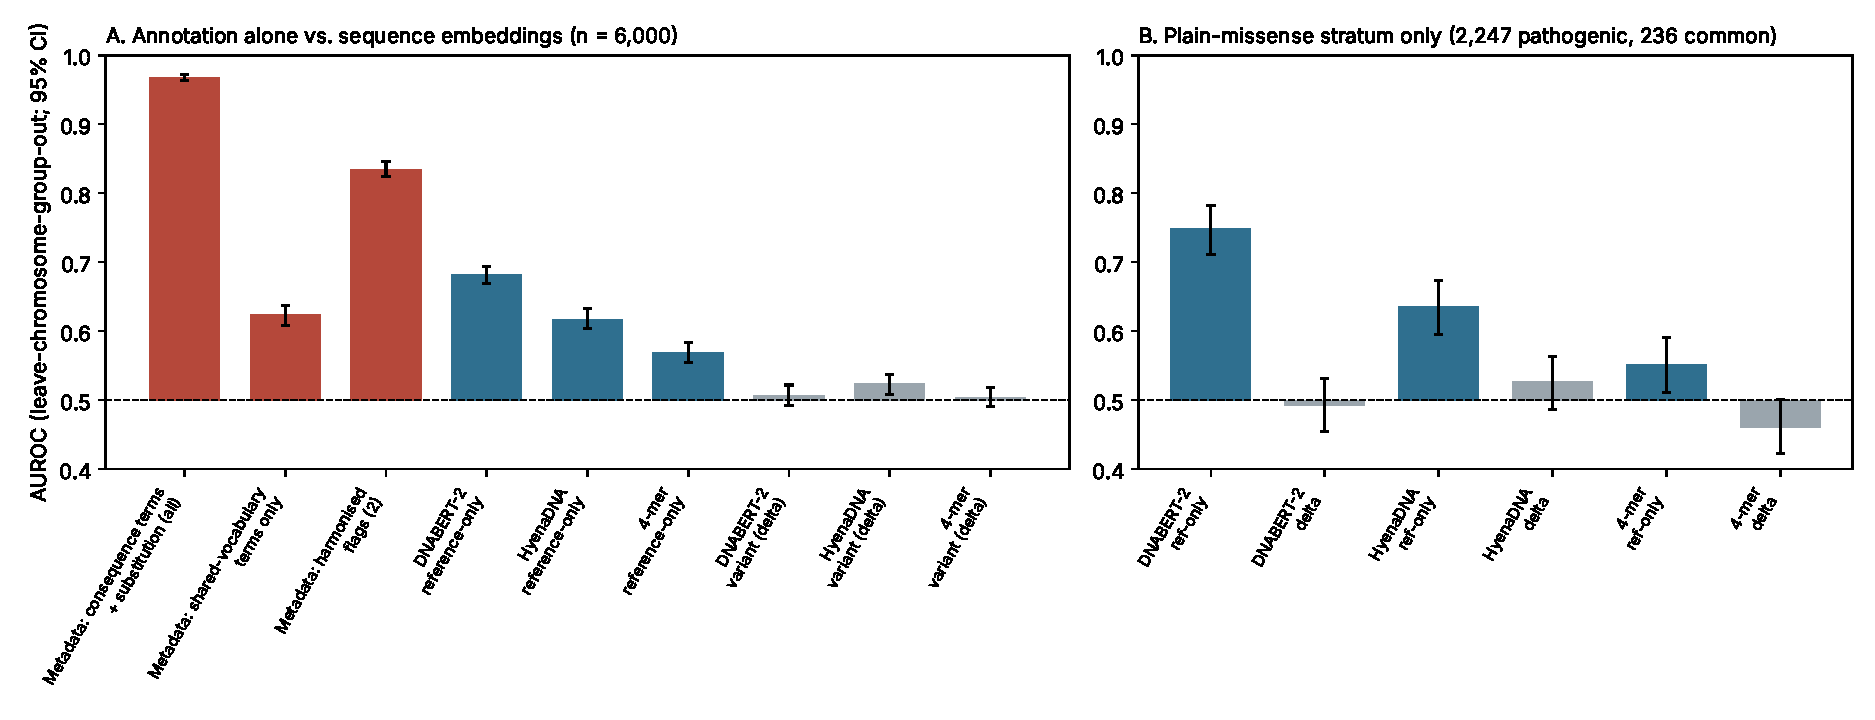
\includegraphics[width=\linewidth]{generated/fig_leakage_main.pdf}
\caption{(A)~AUROC of annotation-only probes (red), reference-only embeddings (blue) and variant ($\Dlt$) embeddings (grey) for all \NSample{} variants; error bars are 95\% bootstrap intervals. (B)~The same embedding probes restricted to plain-missense variants (\PureStratP{} pathogenic, \PureStratC{} common), where annotation carries little information. The dashed line marks chance.}
\label{fig:main}
\end{figure}

\subsection{Variant-specific embeddings are close to chance}
The variant-specific ($\Dlt$) probes reached AUROC \DnbDelta{} (DNABERT-2), \HynDelta{} (HyenaDNA) and \KmDelta{} (4-mer), all within about 0.03 of chance, and did not rise above chance in any stratum (Table~\ref{tab:strata}). Label-shuffling gave a mean AUROC of \ShufMean{} (maximum \ShufMax{} over 40 permutations), so the pipeline itself is not producing spurious signal. The median relative size of the alternate-minus-reference difference was \RelHyn\% (HyenaDNA), \RelDnb\% (DNABERT-2) and \RelAg\% (AlphaGenome) of the reference embedding norm, so a one-base change is a small perturbation of a pooled representation, a point we return to below.

\subsection{What remains once annotation is removed}
Within plain-missense variants, annotation metadata carries little information (substitution type alone gives AUROC \MetaPure{} there), yet reference-only embeddings remained informative: DNABERT-2 \DnbRefPure{} \ci{\DnbRefPureLo}{\DnbRefPureHi}, HyenaDNA \HynRefPure{} \ci{\HynRefPureLo}{\HynRefPureHi} and the 4-mer baseline \KmRefPure{} (Table~\ref{tab:strata}; Figure~\ref{fig:main}B). Probes trained within the stratum gave similar values (\DnbRefPureTrained{} and \HynRefPureTrained). Adding the reference-only score to annotation raised AUROC only slightly (DNABERT-2 by \IncDnb{} \ci{\IncDnbLo}{\IncDnbHi}; HyenaDNA by \IncHyn{} \ci{\IncHynLo}{\IncHynHi}). A signal tied to the sequence \emph{around} the variant therefore persists, but it is not the variant: by construction a reference-only score is identical for different alleles at the same position.

\begin{table}[t]
\centering\small
\begin{tabular}{lcc}\toprule
Feature source & Scores from probe trained on & AUROC (95\% CI)\\\midrule
Annotation (substitution type only here) & all 6,000 variants & 0.582 (0.545-0.620)\\
DNABERT-2 reference-only & all 6,000 variants & 0.749 (0.711-0.782)\\
DNABERT-2 reference-only & plain-missense variants only & 0.721 (0.683-0.757)\\
DNABERT-2 variant ($\Delta$) & all 6,000 variants & 0.493 (0.455-0.532)\\
HyenaDNA reference-only & all 6,000 variants & 0.635 (0.596-0.674)\\
HyenaDNA reference-only & plain-missense variants only & 0.649 (0.609-0.688)\\
HyenaDNA variant ($\Delta$) & all 6,000 variants & 0.527 (0.487-0.563)\\
4-mer reference-only & all 6,000 variants & 0.552 (0.512-0.591)\\
4-mer variant ($\Delta$) & all 6,000 variants & 0.460 (0.422-0.501)\\
\bottomrule\end{tabular}

\caption{Plain-missense stratum (\PureStratP{} pathogenic, \PureStratC{} common). With only \PureStratC{} common variants, intervals are wide and the stratum should be read as supporting, not definitive, evidence. The annotation row reflects substitution type only because consequence strings are identical within the stratum. All strata are in Supplementary Table~S4.}
\label{tab:strata}
\end{table}

\subsection{Robustness}
Chromosome-cluster intervals were similar to the bootstrap intervals (Table~\ref{tab:main}) and fold-level AUROCs were consistent across the three chromosome groups (Supplementary Table~S1). Restricting pathogenic variants to those with assertion criteria, or to multiple-submitter and expert-panel assertions, left every result essentially unchanged (annotation alone \RevAnnMin-\RevAnnMax; Supplementary Table~S3), so the findings are not driven by the weakest ClinVar assertions. The annotation result (AUROC \CAnnMin-\CAnnMax) and the near-chance variant results (\CDeltaMin-\CDeltaMax) were stable across probe regularisation strengths, whereas reference-only AUROC varied (DNABERT-2 \CRefDnbMin-\CRefDnbMax; HyenaDNA \CRefHynMin-\CRefHynMax; Supplementary Table~S2); we report $C=1$ throughout, chosen in advance, and none of the conclusions depends on this choice.

\subsection{AlphaGenome subset}
In the separate \AgN-variant subset, annotation alone again reached \AgMeta{} \ci{\AgMetaLo}{\AgMetaHi}, the reference-only embedding \AgRef{} \ci{\AgRefLo}{\AgRefHi} and the variant ($\Dlt$) embedding \AgDelta{} \ci{\AgDeltaLo}{\AgDeltaHi} (Table~\ref{tab:ag}). These numbers are not comparable with the other models, because the subset is small, lies entirely on one chromosome and uses position-block folds; we report it as an independent confirmation of the pattern, not as a ranking.

\begin{table}[t]
\centering\small
\begin{tabular}{lc}\toprule
Feature source (1,018 variants; position-block CV) & AUROC (95\% CI)\\\midrule
Annotation: consequence terms + substitution & 0.959 (0.945--0.970)\\
AlphaGenome reference-only & 0.608 (0.573--0.643)\\
AlphaGenome variant ($\Delta$) & 0.514 (0.481--0.552)\\
\bottomrule\end{tabular}

\caption{AlphaGenome validation subset (\AgPath{} pathogenic, \AgCommon{} common variants; all on chromosome~8; five position-block folds). Not comparable with Table~\ref{tab:main}.}
\label{tab:ag}
\end{table}

% =============================================================================
\section{Discussion}
\textbf{Principal findings.} Annotation metadata alone, with no DNA sequence, reached AUROC \MetaAll{} and outperformed every genomic AI embedding we evaluated (best: \DnbRef). The effect of the substitution on model embeddings was close to chance. The headline accuracy of a sequence-based classifier on this task can therefore not be taken as evidence that it understands variant effects. A residual locus-level signal exists in reference-sequence embeddings, most clearly for DNABERT-2, but it cannot by itself discriminate between variants at the same locus.

\textbf{Why shortcut-driven accuracy is misleading for computational evidence.} The PP3 and BP4 criteria assume that a tool's output reflects something about the variant's effect, and the strength of evidence assigned to a score depends on its calibration against variants not used to build the tool \citep{richards2015acmg,pejaver2022calibration}. Shortcut-driven accuracy undermines this in three ways. First, a shortcut that is present in a benchmark is typically absent in a diagnostic laboratory, where every candidate variant has been annotated by the same pipeline; the performance measured on the benchmark then overstates the performance obtainable in the clinic. Second, evidence strength is derived from measured accuracy, so inflated accuracy leads to over-weighted evidence. Third, features that correlate with annotation (for example, transcript type or gene) are partly information the classifier already has, creating a risk of counting the same evidence twice. The reference-only result is the genomic analogue of a well-described problem: tools can learn which genes or loci tend to harbour pathogenic variants rather than which variants are pathogenic \citep{grimm2015circularity}. The clinically hard problem, deciding which variant \emph{within} a gene is pathogenic, is exactly the one a reference-only score cannot address.

\textbf{Reporting checklist.} The most useful takeaway of this audit is practical. Table~\ref{tab:checklist} lists seven items that a benchmark of AI-assisted variant interpretation should report. They are inexpensive, require no new model, and align with general reporting guidance for prediction models that use machine learning \citep{collins2024tripod}.

\begin{table}[t]
\centering\small
\begin{tabularx}{\linewidth}{@{}c>{\raggedright\arraybackslash}p{4.9cm}>{\raggedright\arraybackslash}X@{}}
\toprule
 & Report & Why (finding in this study)\\\midrule
1 & An annotation-only baseline built from every metadata field available for both classes & Annotation alone reached AUROC \MetaAll{} versus \DnbRef{} for the best embedding\\
2 & A class-by-term table of annotation vocabulary, and confirmation that both classes were annotated by one pipeline and version & Several terms occurred in one class only, including a misspelt term\\
3 & A context-only (reference-sequence) control & Reference-only embeddings out-performed variant-specific ones by up to \DnbSens{} AUROC\\
4 & The variant-specific signal on its own ($\Dlt$ or an equivalent), reported next to the headline metric & Variant-specific embeddings were within about 0.03 of chance\\
5 & Results in matched or stratified subsets, with per-class counts and intervals & Plain-missense stratum has only \PureStratC{} common variants; conclusions there are tentative\\
6 & Held-out chromosomes or loci, with intervals that account for clustering & Chromosome-cluster intervals were reported alongside bootstrap intervals\\
7 & The intended use, the data on which accuracy was measured, and an explicit statement that benchmark accuracy is not evidence for clinical use & The benchmark is balanced and retrospective\\
\bottomrule
\end{tabularx}
\caption{Reporting checklist for benchmarks of AI-assisted variant interpretation.}
\label{tab:checklist}
\end{table}

\textbf{Implications for public health.} Variant classification underpins diagnosis, cascade testing of relatives and reproductive decisions. The people affected when a computational score is over-weighted are therefore patients and their families, and the clinical laboratories that must later reclassify variants, at cost to both. As AI-assisted tools enter these workflows, reliability depends on evaluations that are transparent and reproducible, and on users being able to see what a reported accuracy does and does not demonstrate. Our results argue for independent, benchmark-agnostic validation before computational scores are given weight as evidence, and for benchmark maintainers to annotate all classes with a single pipeline. Reliable evaluation of AI tools is a prerequisite for equitable genetic testing; the audit and checklist offered here give developers and laboratories a concrete, inexpensive check to run before a tool is relied on.

\textbf{Relation to prior work.} Large benchmarking efforts report that model rankings are unstable and that representations depend on the downstream task and on how embeddings are summarised \citep{feng2025benchmark,tang2025representational,ledneva2026geneb}. Our work is complementary: it does not rank models, and instead asks whether the benchmark measures what it is taken to measure. The control we use follows the logic of control tasks for probes \citep{hewitt2019control}.

\subsection*{Limitations}
These results show what this benchmark measures; they do not test what the models can represent. (1)~Scope: this audit examines one published benchmark and one task; the same checks can be applied to other variant benchmarks. (2)~The class-balanced sample (\NPerClass{} variants per class) does not reflect clinical prevalence. (3)~The plain-missense stratum contains \PureStratC{} common variants (48 in the AlphaGenome subset, which also lies on one chromosome and uses position-block folds) that are not a random sample of common variation, so estimates there are imprecise; they support, and do not drive, the main result. (4)~The cause of the vocabulary difference is a question for the benchmark's maintainers; the pattern is consistent with different annotation tools or versions. (5)~The source of the residual reference-only signal is an open question that a gene-held-out analysis could address once benchmarks provide gene identifiers; candidate explanations include gene identity, evolutionary constraint and sequence composition. (6)~We evaluate the widely used frozen-embedding setting, mean-pooled embeddings with linear probes, which measures readily accessible information; pooling at the variant position and intermediate layers were not tested, and the variant perturbation is small (\RelHyn\%, \RelDnb\% and \RelAg\% of the embedding norm for HyenaDNA, DNABERT-2 and AlphaGenome), so conclusions concern this evaluation setting. (7)~The three main models represent three families (a transformer, a long-convolution model and a non-neural baseline); the conclusions concern the benchmark, not model architectures. (8)~Nothing here has been validated clinically, and none of the models or probes is intended for clinical use.

% =============================================================================
\section{Conclusion}
On a published pathogenic-versus-common missense benchmark, annotation metadata alone, with no DNA sequence, reached AUROC \MetaAll{} and outperformed every genomic AI embedding we evaluated (best: \DnbRef), while variant-specific embeddings performed near chance. Benchmark accuracy of this kind is therefore not evidence of understanding variant effects, and it should not be used to justify weight for computational evidence in variant classification. We recommend that benchmarks of AI-assisted variant interpretation report an annotation-only baseline, a context-only control and stratified results, as set out in the checklist above. Transparent, benchmark-independent validation should accompany any AI tool before it informs patient care.

\section*{Data and code availability}
Variants derive from the public benchmark of \citet{feng2025benchmark}. Code, per-variant out-of-fold scores and all result tables are available at \url{https://github.com/willhhx/variant-benchmark-audit}.

% APA 7th edition reference list (hand-formatted; keys match refs.bib).
% Page ranges use a hyphen to match the manuscript's dash convention (APA 7 itself specifies an en dash).
\begin{thebibliography}{21}
\setlength{\itemsep}{0pt}

\bibitem[{Avsec et~al.(2026)}]{avsec2026alphagenome}
Avsec, {\v Z}., Latysheva, N., Cheng, J., Novati, G., Taylor, K. R., Ward, T., Bycroft, C., Nicolaisen, L., Arvaniti, E., Pan, J., Thomas, R., Dutordoir, V., Perino, M., De, S., Karollus, A., Gayoso, A., Sargeant, T., Mottram, A., Wong, L. H., \ldots{} Kohli, P. (2026). Advancing regulatory variant effect prediction with AlphaGenome. \textit{Nature}, \textit{649}(8099), 1206-1218. \url{https://doi.org/10.1038/s41586-025-10014-0}

\bibitem[{Benegas et~al.(2023)}]{benegas2023gpn}
Benegas, G., Batra, S. S., \& Song, Y. S. (2023). DNA language models are powerful predictors of genome-wide variant effects. \textit{Proceedings of the National Academy of Sciences}, \textit{120}(44), Article e2311219120. \url{https://doi.org/10.1073/pnas.2311219120}

\bibitem[{Bredikhin et~al.(2026)}]{bredikhin2026alphagenomepytorch}
Bredikhin, D., Kjellberg, M., Zou, C., Buendia, A., Tu, X., \& Kundaje, A. (2026). \textit{alphagenome-pytorch: A PyTorch port of AlphaGenome} (Version 0.3.1) [Computer software]. GitHub. \url{https://github.com/genomicsxai/alphagenome-pytorch}

\bibitem[{Collins et~al.(2024)}]{collins2024tripod}
Collins, G. S., Moons, K. G. M., Dhiman, P., Riley, R. D., Beam, A. L., Van Calster, B., Ghassemi, M., Liu, X., Reitsma, J. B., van Smeden, M., Boulesteix, A.-L., Camaradou, J. C., Celi, L. A., Denaxas, S., Denniston, A. K., Glocker, B., Golub, R. M., Harvey, H., Heinze, G., \ldots{} Logullo, P. (2024). TRIPOD+AI statement: Updated guidance for reporting clinical prediction models that use regression or machine learning methods. \textit{BMJ}, \textit{385}, Article e078378. \url{https://doi.org/10.1136/bmj-2023-078378}

\bibitem[{Efron \& Tibshirani(1993)}]{efron1993bootstrap}
Efron, B., \& Tibshirani, R. J. (1993). \textit{An introduction to the bootstrap}. Chapman \& Hall.

\bibitem[{Feng et~al.(2025)}]{feng2025benchmark}
Feng, H., Wu, L., Zhao, B., Huff, C., Zhang, J., Wu, J., Lin, L., Wei, P., \& Wu, C. (2025). Benchmarking DNA foundation models for genomic and genetic tasks. \textit{Nature Communications}, \textit{16}, Article 10780. \url{https://doi.org/10.1038/s41467-025-65823-8}

\bibitem[{Geirhos et~al.(2020)}]{geirhos2020shortcut}
Geirhos, R., Jacobsen, J.-H., Michaelis, C., Zemel, R., Brendel, W., Bethge, M., \& Wichmann, F. A. (2020). Shortcut learning in deep neural networks. \textit{Nature Machine Intelligence}, \textit{2}, 665-673. \url{https://doi.org/10.1038/s42256-020-00257-z}

\bibitem[{Grimm et~al.(2015)}]{grimm2015circularity}
Grimm, D. G., Azencott, C.-A., Aicheler, F., Gieraths, U., MacArthur, D. G., Samocha, K. E., Cooper, D. N., Stenson, P. D., Daly, M. J., Smoller, J. W., Duncan, L. E., \& Borgwardt, K. M. (2015). The evaluation of tools used to predict the impact of missense variants is hindered by two types of circularity. \textit{Human Mutation}, \textit{36}(5), 513-523. \url{https://doi.org/10.1002/humu.22768}

\bibitem[{Hewitt \& Liang(2019)}]{hewitt2019control}
Hewitt, J., \& Liang, P. (2019). Designing and interpreting probes with control tasks. In \textit{Proceedings of the 2019 Conference on Empirical Methods in Natural Language Processing and the 9th International Joint Conference on Natural Language Processing (EMNLP-IJCNLP)} (pp. 2733-2743). Association for Computational Linguistics. \url{https://doi.org/10.18653/v1/D19-1275}

\bibitem[{Kao et~al.(2024)}]{kao2024lrb}
Kao, C.-H., Trop, E., Polen, M., Schiff, Y., de Almeida, B. P., Gokaslan, A., Pierrot, T., \& Kuleshov, V. (2024). Advancing DNA language models: The genomics long-range benchmark. In \textit{ICLR 2024 Workshop on Machine Learning for Genomics Explorations}. \url{https://mlanthology.org/iclrw/2024/kao2024iclrw-advancing/}

\bibitem[{Kapoor \& Narayanan(2023)}]{kapoor2023leakage}
Kapoor, S., \& Narayanan, A. (2023). Leakage and the reproducibility crisis in machine-learning-based science. \textit{Patterns}, \textit{4}(9), Article 100804. \url{https://doi.org/10.1016/j.patter.2023.100804}

\bibitem[{Karczewski et~al.(2020)}]{karczewski2020gnomad}
Karczewski, K. J., Francioli, L. C., Tiao, G., Cummings, B. B., Alf{\"o}ldi, J., Wang, Q., Collins, R. L., Laricchia, K. M., Ganna, A., Birnbaum, D. P., Gauthier, L. D., Brand, H., Solomonson, M., Watts, N. A., Rhodes, D., Singer-Berk, M., England, E. M., Seaby, E. G., Kosmicki, J. A., \ldots{} MacArthur, D. G. (2020). The mutational constraint spectrum quantified from variation in 141,456 humans. \textit{Nature}, \textit{581}(7809), 434-443. \url{https://doi.org/10.1038/s41586-020-2308-7}

\bibitem[{Landrum et~al.(2018)}]{landrum2018clinvar}
Landrum, M. J., Lee, J. M., Benson, M., Brown, G. R., Chao, C., Chitipiralla, S., Gu, B., Hart, J., Hoffman, D., Jang, W., Karapetyan, K., Katz, K., Liu, C., Maddipatla, Z., Malheiro, A., McDaniel, K., Ovetsky, M., Riley, G., Zhou, G., \ldots{} Maglott, D. R. (2018). ClinVar: Improving access to variant interpretations and supporting evidence. \textit{Nucleic Acids Research}, \textit{46}(D1), D1062-D1067. \url{https://doi.org/10.1093/nar/gkx1153}

\bibitem[{Ledneva et~al.(2026)}]{ledneva2026geneb}
Ledneva, D., Nuridinov, M., \& Kuznetsov, D. (2026). \textit{GENEB: Why genomic models are hard to compare} [Preprint]. arXiv. \url{https://arxiv.org/abs/2606.04525}

\bibitem[{Nguyen et~al.(2023)}]{nguyen2023hyenadna}
Nguyen, E., Poli, M., Faizi, M., Thomas, A., Birch-Sykes, C., Wornow, M., Patel, A., Rabideau, C., Massaroli, S., Bengio, Y., Ermon, S., Baccus, S. A., \& R{\'e}, C. (2023). HyenaDNA: Long-range genomic sequence modeling at single nucleotide resolution. In \textit{Advances in Neural Information Processing Systems} (Vol. 36). Curran Associates. \url{https://proceedings.neurips.cc/paper_files/paper/2023/hash/86ab6927ee4ae9bde4247793c46797c7-Abstract-Conference.html}

\bibitem[{Pedregosa et~al.(2011)}]{pedregosa2011sklearn}
Pedregosa, F., Varoquaux, G., Gramfort, A., Michel, V., Thirion, B., Grisel, O., Blondel, M., Prettenhofer, P., Weiss, R., Dubourg, V., Vanderplas, J., Passos, A., Cournapeau, D., Brucher, M., Perrot, M., \& Duchesnay, {\'E}. (2011). Scikit-learn: Machine learning in Python. \textit{Journal of Machine Learning Research}, \textit{12}, 2825-2830. \url{https://jmlr.org/papers/v12/pedregosa11a.html}

\bibitem[{Pejaver et~al.(2022)}]{pejaver2022calibration}
Pejaver, V., Byrne, A. B., Feng, B.-J., Pagel, K. A., Mooney, S. D., Karchin, R., O'Donnell-Luria, A., Harrison, S. M., Tavtigian, S. V., Greenblatt, M. S., Biesecker, L. G., Radivojac, P., \& Brenner, S. E. (2022). Calibration of computational tools for missense variant pathogenicity classification and ClinGen recommendations for PP3/BP4 criteria. \textit{American Journal of Human Genetics}, \textit{109}(12), 2163-2177. \url{https://doi.org/10.1016/j.ajhg.2022.10.013}

\bibitem[{Richards et~al.(2015)}]{richards2015acmg}
Richards, S., Aziz, N., Bale, S., Bick, D., Das, S., Gastier-Foster, J., Grody, W. W., Hegde, M., Lyon, E., Spector, E., Voelkerding, K., Rehm, H. L., \& ACMG Laboratory Quality Assurance Committee. (2015). Standards and guidelines for the interpretation of sequence variants: A joint consensus recommendation of the American College of Medical Genetics and Genomics and the Association for Molecular Pathology. \textit{Genetics in Medicine}, \textit{17}(5), 405-424. \url{https://doi.org/10.1038/gim.2015.30}

\bibitem[{Tang \& Koo(2025)}]{tang2025representational}
Tang, Z., \& Koo, P. K. (2025). Evaluating the representational power of pre-trained DNA language models for regulatory genomics. \textit{Genome Biology}. \url{https://doi.org/10.1186/s13059-025-03674-8}

\bibitem[{Tavtigian et~al.(2018)}]{tavtigian2018bayesian}
Tavtigian, S. V., Greenblatt, M. S., Harrison, S. M., Nussbaum, R. L., Prabhu, S. A., Boucher, K. M., \& Biesecker, L. G. (2018). Modeling the ACMG/AMP variant classification guidelines as a Bayesian classification framework. \textit{Genetics in Medicine}, \textit{20}(9), 1054-1060. \url{https://doi.org/10.1038/gim.2017.210}

\bibitem[{Zhou et~al.(2024)}]{zhou2024dnabert2}
Zhou, Z., Ji, Y., Li, W., Dutta, P., Davuluri, R. V., \& Liu, H. (2024). DNABERT-2: Efficient foundation model and benchmark for multi-species genomes. In \textit{The Twelfth International Conference on Learning Representations}. \url{https://iclr.cc/virtual/2024/poster/17823}

\end{thebibliography}


\end{document}
